\section{Proof of concept implementation for health data sharing}
\label{sec:poc_health}

In this Section, a proof of concept implementation of the proposed algorithms for offer instantiation and policy matching towards the generation of a data access agreement is described for a specific use case involving health data sharing.

\subsection{Background and motivation}
\label{sec:poc_background}

In this Thesis, a health data sharing use case was selected to showcase the strengths of the proposed algorithm since the exchange of health-related data presents significant potential for advancing research and leveraging advanced computational and statistical techniques to drive progress in healthcare.
However, due to its sensitive nature and potentially significant impact if misused, the sharing and utilisation of health-related data are highly regulated at both legal and institutional levels, e.g., \textit{``data concerning health''} is a special category of personal data under the GDPR, i.e., Article 9.1~\citeyearpar{noauthor_regulation_2016}, and as such its processing is prohibited unless one of the legal grounds of Article 9.2 applies.

Currently, institutions such as hospitals handle each health data request through a dedicated committee tasked with evaluating and making decisions regarding the release of such data under their care.
To facilitate this process, the Global Alliance for Genomics and Health\footnote{\url{https://www.ga4gh.org/} (accessed on 2 April 2024)} (GA4GH) was established as an international consortium focused on the development of standards and the promotion of responsible sharing of genomics and health data.
Among its various resources, aimed at different aspects and processes of health-related data sharing, GA4GH has introduced a machine-readable ontology known as the Data Use Ontology\footnote{\url{http://purl.obolibrary.org/obo/duo} (accessed on 2 April 2024)} (DUO).
DUO~\citep{lawson_data_2021,rehm_ga4gh_2021} was designed to express Data Use Limitations (DULs), i.e., conditions and constraints defined by data providers which should be respected by data requesters to use said data.

DUO is an OWL ontology aligned with the Open Biological and Biomedical Ontology\footnote{\url{https://obofoundry.org/} (accessed on 2 April 2024)} (OBO).
By utilising OBO's upper level ontologies, DUO ensures semantic interoperability with a range of biomedical ontologies belonging to the OBO family of ontologies.
As such, DUO's main purpose is related to annotating datasets with DUL codes to specify usage conditions, articulate data usage requests, and automatically identify or discover compatible datasets by comparing requests with datasets' usage conditions.

\paragraph{DUO and existing efforts}
DUO concepts are organised into three taxonomies:
\begin{enumerate}
    \item The `Data Use Permission' taxonomy, denoted by the base class \texttt{obo:DUO\_0000001}, encompasses permissions related to purposes for data usage.
    \item The `Data Use Modifier' taxonomy, denoted by the base class \texttt{obo:DUO\_0000017}, covers additional conditions to be applied alongside data use permissions.
    \item The `Investigation' taxonomy, denoted by the base class \texttt{obo:OBI\_0000066} from the Ontology for Biomedical Investigations\footnote{\url{http://obi-ontology.org/} (accessed on 3 April 2024)} (OBI), delineates planned conditions for which data is being requested.
\end{enumerate}
Furthermore, the \texttt{obo:DUO\_0000010} property implements a \textit{`is restricted to'} relation, used to limit certain concepts to certain contexts, e.g., to restrict the \texttt{obo:DUO\_0000022} concept, which indicates usage permitted within a geographic region, to terms from \texttt{obo:GAZ\_00000448}, the base concept from the Gazetteer (places) ontology\footnote{\url{https://environmentontology.github.io/gaz/} (accessed on 3 April 2024)}.

DUO originated from prior endeavours aimed at establishing consent codes for data usage and leveraging them as machine-readable information for automated access to data.
Its initial development drew upon the Consent Codes by \cite{dyke_consent_2016}, which specified concepts for data usage based on consent permissions.
Subsequently, DUO incorporated a few terms from the Automatable Discovery and Access Matrix (ADA-M) framework \citep{woolley_responsible_2018}, which shares akin objectives and concepts.
As such, the intended utilisation of DUO revolves around facilitating the recording of consent for sharing and reusing biomedical datasets, as outlined by \cite{lawson_data_2021} and \cite{rehm_ga4gh_2021}, the latter highlighting the usage of DUO in distinct GA4GH initiatives.

The Data Use Oversight System\footnote{\url{https://duos.broadinstitute.org/} (accessed on 2 April 2024)} (DUOS) is a platform built upon DUO aimed at facilitating semi-automated management of access health-related datasets.
It leverages DUO annotations to incorporate new datasets and data access requests, which are subsequently matched using an algorithm based on hierarchical compatibility.
Figure~\ref{fig:duo-matching} illustrates the algorithm followed by this platform, where the `Data Use Codes' correspond to concepts from the previously mentioned DUO `Data Use Permission' taxonomy,  the `Data Use Requirements' to the `Data Use Modifier' taxonomy, and the `Research Purpose Terms/Data Use Categories' to the `Investigation' taxonomy.
This algorithm entails matching the dataset's access conditions with the data requester's conditions by relying on the subclass relations between them.
The results of this matching algorithm are then reviewed by a `Data Access Committee' to finalise the conditions of the access agreement and provide the data requested with access to the relevant datasets, comparable with the decision-making processes of human data access committees \citep{cabili_empirical_2021}.
The NHGRI Genomic Data Science Analysis, Visualization, and Informatics Lab-space project\footnote{\url{https://anvilproject.org} (accessed on 3 April 2024)} implemented a large-scale pilot using the DUOS platform implementation \citep{schatz_inverting_2022}.

\begin{figure}[ht]
    \centering
    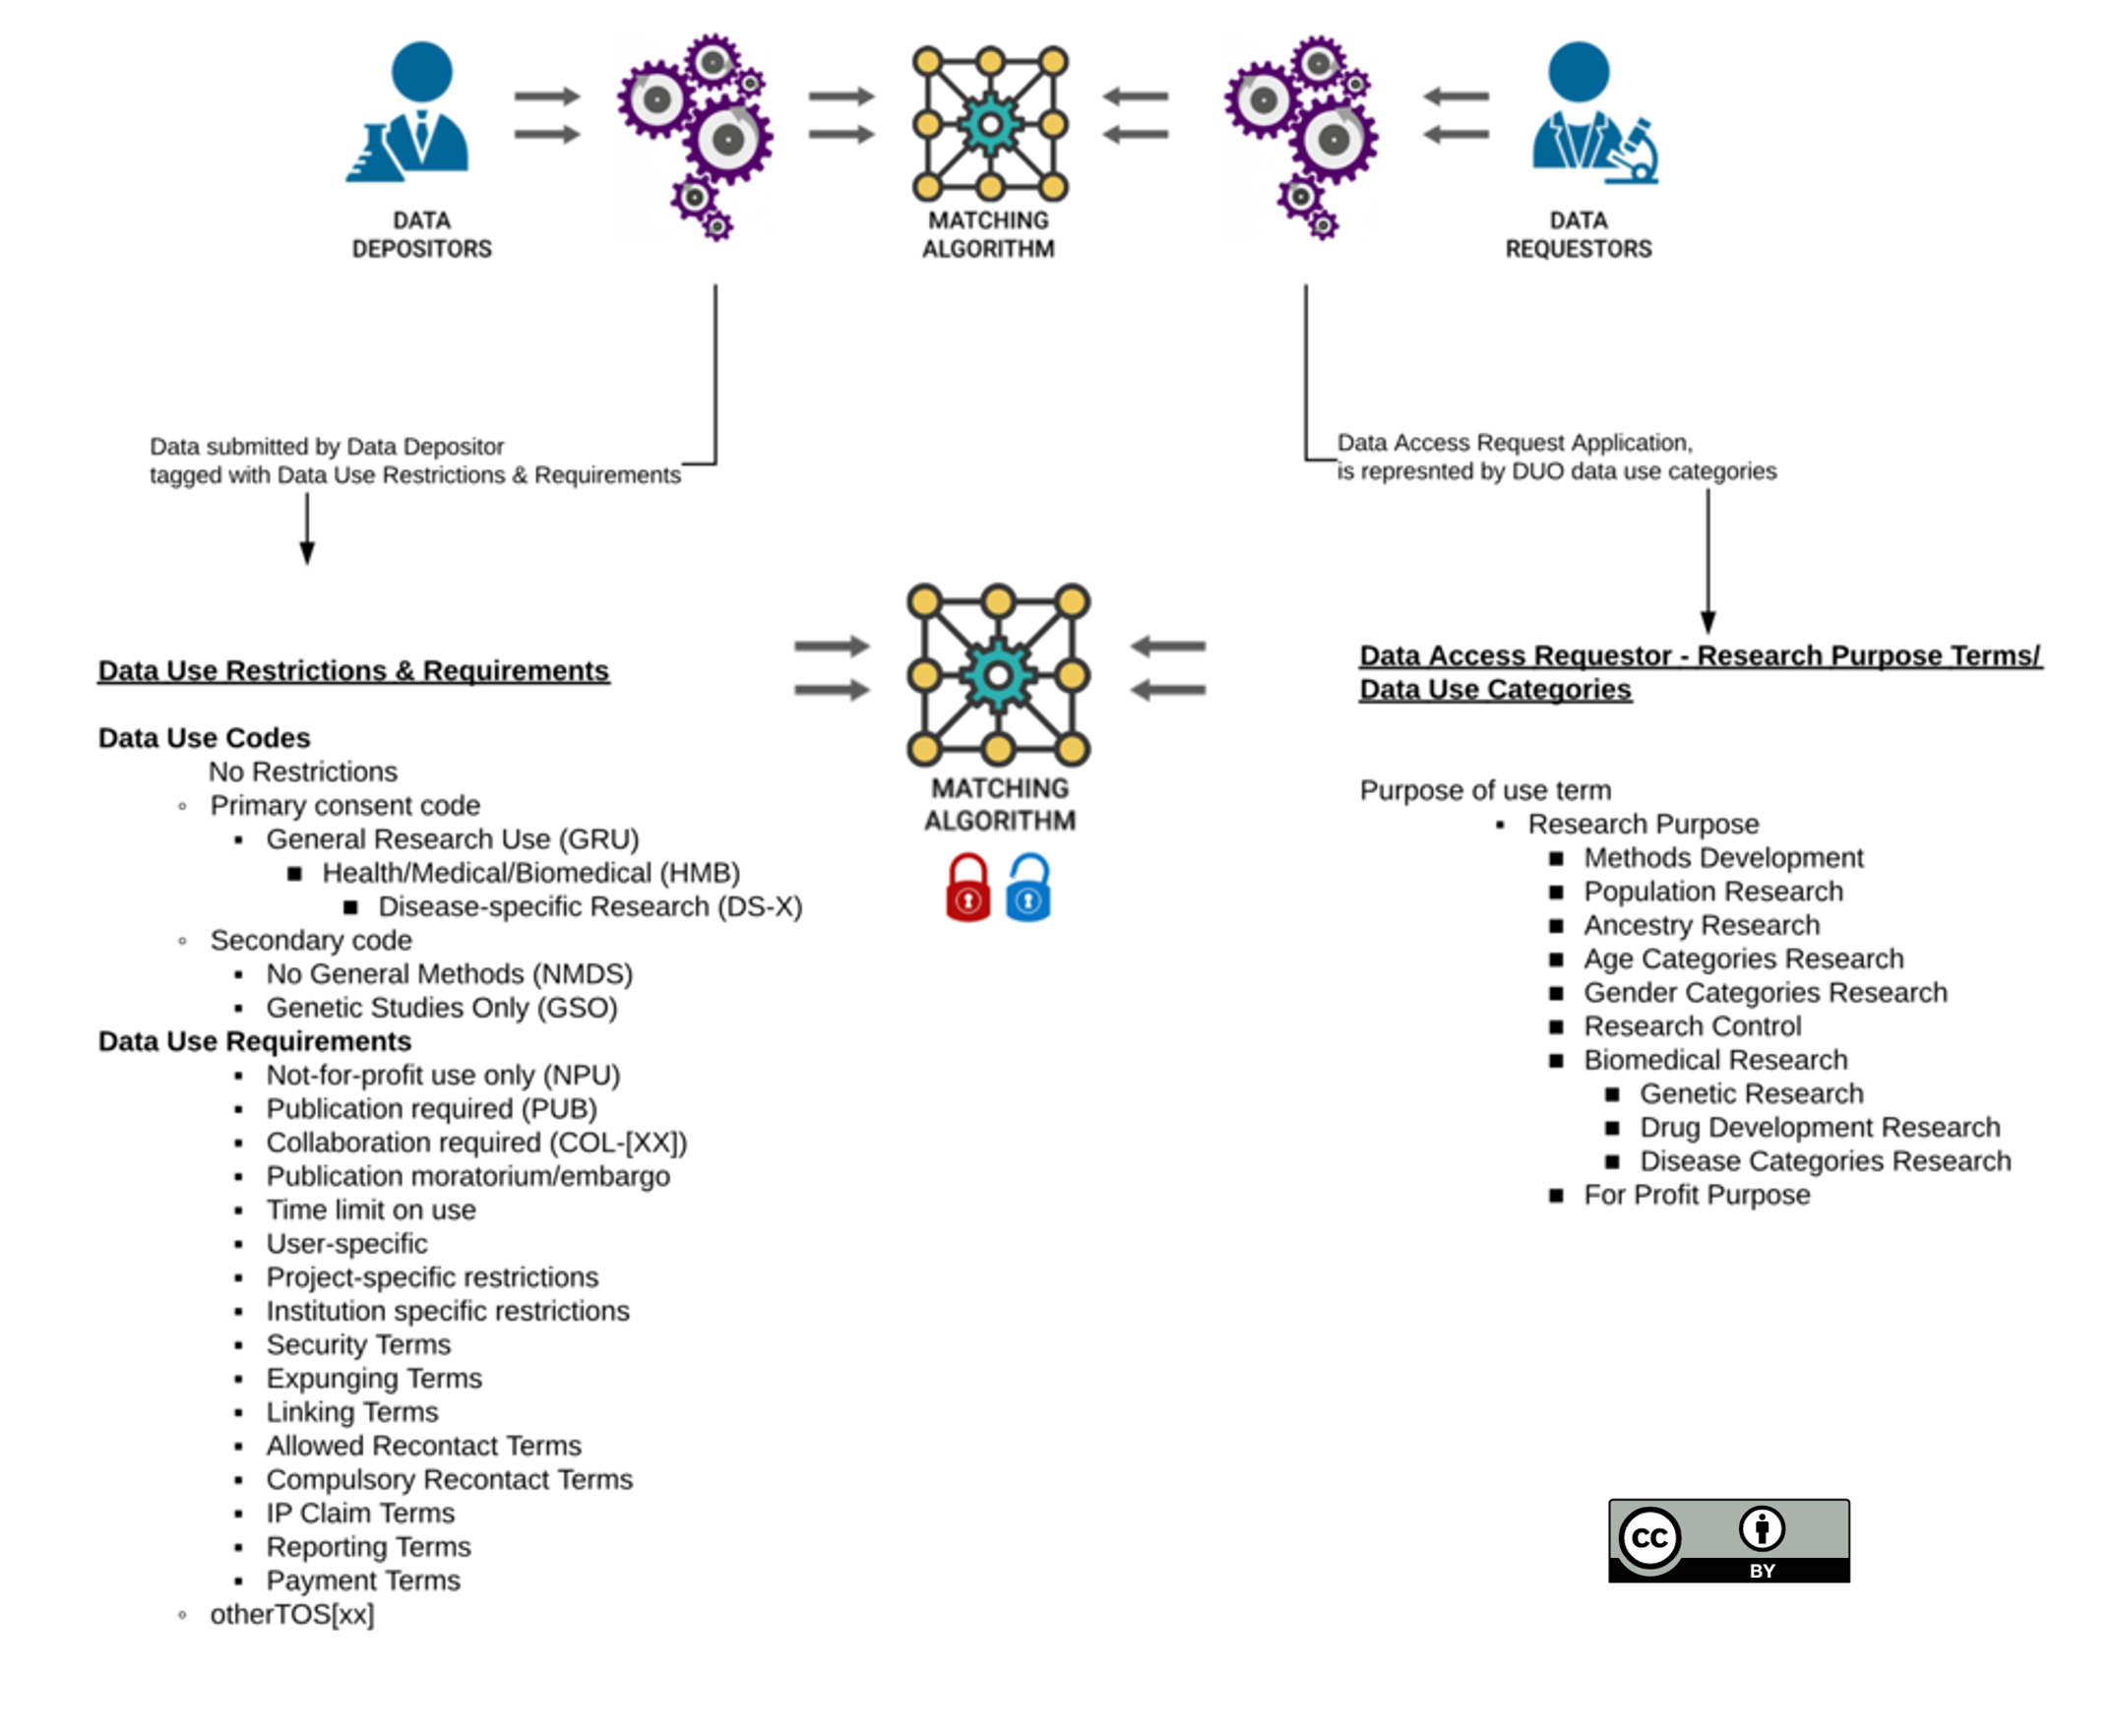
\includegraphics[width=1\linewidth]{figures//chapter-6/DUO-matching-with-license.png}
    \caption{DUO-based matching algorithm, adapted from \url{https://github.com/EBISPOT/DUO}.}
    \label{fig:duo-matching}
\end{figure}

Beyond DUOS, the DUO specification has been integrated into various other works, including a specification of informed consent for health and genomics research in Africa \citep{nembaware_framework_2019}, a blockchain-based consent model for health data sharing \citep{jaiman_consent_2020}, and an online platform that offers dynamic consent interfaces and tools for large-scale genomics research programs \citep{haas_ctrl_2021}.
Furthermore, DUO is mentioned in the Data Tags Suite (DATS), where it is considered a candidate vocabulary within its framework for discovering metadata-based data access conditions \citep{alter_data_2020}.
Additionally, it plays a role in the roadmap of European infrastructures for accessing a large number of human genomes  \citep{saunders_leveraging_2019}.
Moreover, \cite{amith_expressing_2022} demonstrate the usage of DUO for the representation of consent metadata, employing SWRL\footnote{\url{https://www.w3.org/Submission/SWRL/} (accessed on 3 April 2024)} to execute permissive rules, and \cite{grabus_landscape_2019} provide a comprehensive overview of rights and licensing initiatives, approaches, and tools for health data sharing, including DUO.

\paragraph{Challenges of the DUO specification}
DUO expresses DULs as concepts with human-readable definitions, utilising the \texttt{obo:IAO\_0000115} property, e.g., as \texttt{skos:definition} is used to define SKOS concepts.
This limits their utility to humans or machines that operate solely on known concepts.
Furthermore, DUO concepts lack linkage to relevant legal concepts, leading to ambiguity regarding the implications of their usage in strongly legislated jurisdictions like the EU, where the GDPR~\citeyearpar{noauthor_regulation_2016} introduces additional accountability and compliance requirements that must be acknowledged and adhered to.
While existing documentation mentions that the applicability of laws falls under the responsibility of the adopter and that DUO terms have not been evaluated for GDPR compliance, it is crucial for data subjects and data controllers to ensure compatibility with existing regulations.
As such, the absence of such support from the DUO specification poses a risk of hindering interoperability as additional approaches need to be taken to fulfil legal requirements.
Moreover, with the EU push to have a common `Health Data Space'\footnote{\url{https://ec.europa.eu/health/ehealth-digital-health-and-care/european-health-data-space_en} (accessed on 2 April 2024)}, machine-readability and automation will play a pivotal role in facilitating legally-aligned health data exchange.

Furthermore, no instructions were found on how to associate DUO conditions with datasets nor on how the data access agreements matching algorithm should work.
While the DUOS framework provides a comprehensive description of how DUO can be utilised, it lacks detailed guidance on the matching algorithm.
DATS \citep{alter_data_2020} also acknowledges the challenge of using DUO for defining permissions and prohibitions, suggesting ODRL as an alternative model for clearer articulation of permissions and prohibitions.

\paragraph{Proposed improvements over the DUO specification}
To achieve \textit{true machine-readability}, DUO concepts must be represented with permissions, prohibitions, constraints, and duties to form machine-readable rules, by leveraging semantic standards for the expression of asset usage conditions.
By formalising the DULs embedded within the descriptions of each DUO concept as a set of rules, these become explicit and can be attached and sent alongside the data for future inspection.

To assess the compatibility of a data request with the dataset's DULs, both the conditions set by the data provider and those articulated by the data requester for data use should be formulated as policies.
These policies can then be matched to determine if the intended use aligns with the dataset's conditions, using the same approach as the one presented in Section~\ref{sec:algorithm}.
While DUO is currently being utilised in this manner, as evidenced in systems like DUOS, the matching relies on hierarchical compatibility between data request and data use conditions established through a subclass relationship, i.e., a data request $DR$ is a subclass/superclass of a data use condition $DUC$.
This approach has limitations in terms of its capacity and expressiveness for delineating fine-grained rules to utilise in automated systems, as not all relevant pieces of information can be explicitly captured in distinct concepts.
For instance, DUO's \texttt{DUO\_0000006} indicates through a sole human-readable label that use is allowed for health/medical/biomedical research purposes, not including the study of population origins or ancestry, while the same information can be much more explicitly declared using ODRL policies with permission and prohibition rules with purpose constraints.

More significantly, in order to automate the generation of data access/usage agreements effectively, a set of criteria should be considered when selecting a vocabulary to articulate such conditions:
\begin{enumerate}
    \item[(i)] the level of expressiveness to define rules and policies, encompassing the ability to express actions, purposes, or other constraints as distinct concepts that can be autonomously specified and evaluated, and combined in distinct ways to represent various types of policies;
    \item[(ii)] the capability to associate and verify their conformity and adherence to legal requirements, e.g., such as the GDPR; and
    \item[(iii)] the capacity to specify access/usage conditions in a machine-readable format and utilise them for assessing the accuracy and comprehensiveness of information that should be in such a data agreement.
\end{enumerate}
% FROM THE PAPER: Such solutions have existed for a while now -- for example, Answer Set Programming (ASP) and logic-based semantic reasoners have been utilised in a variety of domains -- including for representing information and using it for checking legal compliance for GDPR (see Section.\ref{sec:sota-legal}).

With the aforementioned motivation in mind, this Thesis proposes an approach to explicitly represent DUO concepts using RDF, leveraging ODRL and the efforts declared in previous Sections related to an OAC-based architecture for decentralised access to data.
The choice of using ODRL, beyond being a W3C Recommendation for the expression of policies, is supported by the following motives:
\begin{enumerate}
    \item[(i)] it is RDF-based, ensuring machine-readability;
    \item[(ii)] it encompasses concepts that model domain-specific and legally relevant terms to depict constraints, such as spatial and temporal operators, as well as support various types of policies like offers, requests, and agreements; % Additionally, it offers flexibility in utilizing these concepts in a manner analogous to the conventional contents and structures of legal agreements;
    \item[(iii)] its usage can be validated, and efforts are underway within the W3C ODRL CG to actively develop a formal semantics specification~\citep{fornara_odrl_2023};
    \item[(iv)] it facilitates the development of extensions through ODRL profiles, offering the flexibility to tailor ODRL to specific requirements -- as proved by this Thesis' work on OAC (Section~\ref{sec:oac}), which connects ODRL with legal requirements using DPV and can be extended to cater for legal requirements of health data sharing; and
    \item[(v)] backward compatibility can be ensured -- existing DUO-based systems can adopt the practices suggested in this Section and continue being compatible with the DUO specification. Also, DUO users can select which aspects of this solution they want to incorporate into their system.
\end{enumerate}

As such, based on the algorithms described in Section~\ref{sec:algorithm}, in this Section, (i) DUO concepts are modelled as ODRL policies, (ii) such policies are instantiated as ODRL offers for access to health-related datasets, (iii) offers are matched with incoming data requests to generate permissive or prohibitive data agreements, and (iv) work on OAC is recycled to deal with GDPR obligations for the processing of health data.

\subsection{Re-modelling DUO concepts with ODRL}
\label{sec:poc_duodrl}

As outlined in the previous Section, DUO concepts are organised into three taxonomies with textual annotations representing the access conditions.
This Section's main goal is to examine this implicit information and articulate it explicitly as ODRL policies.

Additionally, it aims to ensure compatibility with current and future GA4GH activities, minimising significant disruptions to existing workflows that already use DUO.
% FROM THE PAPER: We consider DUO's primary attractiveness to be the ease with which its concepts can be easily constructed from input mechanisms (such as a form) and simply `tagged' onto a dataset as an annotation. In this, the textual clauses used to describe the concepts are based on well-defined clauses from consent forms\textsuperscript{18}.
Therefore, the role of ODRL is not to supplant DUO but rather to supplement it by providing extra machine-readable information for each DUO concept.
This additional information makes explicit the conditions currently embedded in DUO's textual annotations, enabling them to be validated, matched, and used for data access in an automated fashion.
An ODRL-improved DUO specification can also be used for additional information duties, such as record-keeping by institutions or other legal tasks.
Following the algorithm proposed in Section~\ref{sec:algorithm}, DUO's taxonomies are modelled as ODRL offers and requests and used as inputs of the policy matching algorithm to generate data access agreements.

\paragraph{Identifying ODRL equivalents for DUO concepts}
For each DUO term, the initial task involved discerning the rules and constraints it encompasses, through the analysis of its textual description, to determine whether it should be modelled as a permission, prohibition, or obligation, as well as understanding the specific context in which they should be applied.
With this analysis, the redundancy and overlap between DUO's data use permissions and modifiers is noticeable, as both include purpose-based policies without a clear differentiation in their semantics.
For instance, \texttt{DUO\_0000011} denotes permission, while \texttt{DUO\_0000044} signifies prohibition, both for `population origins or ancestry research' purposes, with the former categorised as a data use permission and the latter a modifier.

Hence, in this Thesis, the restructuring of the DUO taxonomies is proposed by introducing a unique purpose-based taxonomy that models research concepts as ODRL policies, with variants for permissions and prohibitions, and duties applied over permissions with specific research purposes.
% FROM THE PAPER: This is based on DUOS's data collection input forms and ADA-M's concepts where each research purpose can be individually consented (or restricted) to, with possible implications arising from lack of any permission or prohibition.
For instance, the DUO concept for code \texttt{HMB}, which states that ``[t]his data use permission indicates that use is allowed for health / medical / biomedical purposes (HMB); [and] does not include the study of population origins or ancestry'' in its textual definition, should be articulated as being a permission for a purpose of type \texttt{HMB} and not a purpose of type \texttt{POA}.
This approach allows for a more precise expression and application of DUO's \texttt{HMB} concept by revealing its underlying concepts (purpose) and the rules governing it (permission).

Furthermore, upon analysing DUO's concepts and their inherent access conditions, ODRL rules were modelled to represent the conditions of each DUO concept.
In cases where ODRL lacks the necessary concepts, an extension to its existing concepts is proposed to cover the missing ones.
In this context, for each concept, an \texttt{odrl:Set} instance was modelled to represent the DUO concept's intrinsic rules.
These policies are then amalgamated into an \texttt{odrl:Offer}, to serve as a unified policy for a dataset, as detailed in Section \ref{sec:algorithm-offer} regarding the instantiation of offer policies.
A comprehensive compilation of the performed interpretations for each DUO concept is provided in Table \ref{table:DUO_ODRL_overview}.
During this interpretive analysis, difficulties were found in interpreting specific expressions such as `is limited to', a term that suggests that usage is restricted solely within a particular scope.
If this interpretation holds true, DUO developers should clarify how potential conflicts arising from rules expressing exclusive limitations versus other permissive expressions, such as `is allowed for', should be resolved.
Hence, in this Thesis, ODRL's capabilities are used to articulate these requirements as permissions, prohibitions, and obligations, and, subsequently, existing works on ODRL \citep{pellegrini_automated_2018,de_vos_odrl_2019} and OWL \citep{bonatti_realtime_2020} reasoners can be employed to aid solving conflict resolution issues.

\begin{table}[htp]
\caption{Interpretation of DUO concepts' textual descriptions as ODRL policies.}
\label{table:DUO_ODRL_overview}
\footnotesize
\resizebox{\textwidth}{!}{%
\begin{tabular}{p{1.7cm}||p{1.2cm}|p{1.45cm}|p{8.6cm}|p{3.1cm}}
Concept & Code & Rule Type & Constraint & Placeholder \\ \hline\hline
DUO0000001 & \multicolumn{4}{l}{\textbf{Data Use Permission}} \\ \hline\hline
DUO0000042 & GRU & Permission & Purpose is :GRU & ~ \\ \hline
DUO0000006 & HMB & Permission & Purpose is :HMB and not :POA & ~ \\ \hline
DUO0000007 & DS & Permission & Purpose is :DS and mondo:0000001 & :TemplateDisease \\ \hline
DUO0000004 & NRES & Permission & Purpose is odrl:Purpose & ~ \\ \hline
DUO0000011 & POA & Permission & Purpose is :POA & ~ \\ \hline
DUO0000011 & POA & Prohibition & Purpose is not :POA & ~ \\ \hline\hline
DUO0000017 & \multicolumn{4}{l}{\textbf{Data Use Modifier}} \\ \hline\hline
DUO0000043 & CC & Permission & Purpose is :CC & ~ \\ \hline
DUO0000020 & COL & Duty & Action is :CollaborateWithStudyPI & ~ \\ \hline
DUO0000021 & IRB & Duty & Action is :ProvideEthicalApproval & ~ \\ \hline
DUO0000016 & GSO & Permission & Purpose is :GS or :GSG & ~ \\ \hline
DUO0000016 & GSO & Prohibition & Purpose is :GS and not :GSG & ~ \\ \hline
DUO0000022 & GS & Permission & Spatial is equal to specified :Location & :TemplateLocation \\ \hline
DUO0000022 & GS & Prohibition & Spatial is not equal to specified :Location & :TemplateLocation \\ \hline
DUO0000028 & IS & Permission & Assignee is :ApprovedInstitution & :TemplateInstitution \\ \hline
DUO0000028 & IS & Prohibition & Assignee is not :ApprovedInstitution & :TemplateInstitution \\ \hline
DUO0000015 & NMDS & Prohibition & Purpose is :MDS & ~ \\ \hline
DUO0000018 & NPUNCU & Permission & Assignee is :NonProfitOrganisation and Purpose is :NCU & ~ \\ \hline
DUO0000018 & NPUNCU & Prohibition & Assignee is :ForProfitOrganisation and Purpose is :NCU & ~ \\ \hline
DUO0000018 & NPUNCU & Prohibition & Assignee is :NonProfitOrganisation and Purpose is not :NCU & ~ \\ \hline
DUO0000046 & NCU & Permission & Purpose is :NCU & ~ \\ \hline
DUO0000046 & NCU & Prohibition & Purpose is not :NCU & ~ \\ \hline
DUO0000045 & NPU & Permission & Assignee is :NonProfitOrganisation & ~ \\ \hline
DUO0000045 & NPU & Prohibition & Assignee is :ForProfitOrganisation & ~ \\ \hline
DUO0000044 & NPOA & Prohibition & Purpose is :POA & ~ \\ \hline
DUO0000027 & PS & Permission & Project is :ApprovedProject & :TemplateProject \\ \hline
DUO0000027 & PS & Prohibition & Project is not :ApprovedProject & :TemplateProject \\ \hline
DUO0000024 & MOR & Duty & Action is odrl:distribute :ResultsOfStudies with odrl:dateTime & :TemplateDateTime \\ \hline
DUO0000019 & PUB & Duty & Action is odrl:distribute :ResultsOfStudies & ~ \\ \hline
DUO0000012 & RS & Permission & Purpose is specified :Research & :TemplateResearch \\ \hline
DUO0000012 & RS & Prohibition & Purpose is not specified :Research & :TemplateResearch \\ \hline
DUO0000029 & RTN & Duty & Action is :ReturnDerivedOrEnrichedData & ~ \\ \hline
DUO0000025 & TS & Permission & Time is less than specified :TemplateDateTime & :TemplateDateTime \\ \hline
DUO0000026 & US & Permission & Assignee is :ApprovedUser & :TemplateUser \\ \hline
DUO0000026 & US & Prohibition & Assignee is not :ApprovedUser & :TemplateUser \\ \hline\hline
OBI0000066 & \multicolumn{4}{l}{\textbf{Investigation}} \\ \hline\hline
DUO0000034 & & Permission & Purpose is :AgeCategoryResearch & \\ \hline
DUO0000034 & & Permission & Age is specified :Age & :TemplateAgeCategory \\ \hline
DUO0000033 & ~ & Permission & Purpose is :POA & \\ \hline
DUO0000037 & ~ & Permission & Purpose is :HMB & \\ \hline
DUO0000040 & ~ & Permission & Purpose is :DS and mondo:0000001 & :TemplateDisease \\ \hline
DUO0000039 & ~ & Permission & Purpose is :DrugDevelopment & \\ \hline
DUO0000038 & ~ & Permission & Purpose is :GS & \\ \hline
DUO0000035 & ~ & Permission & Purpose is :GenderCategoryResearch & \\ \hline
DUO0000035 & & Permission & Gender is specified :Gender & :TemplateGender \\ \hline
DUO0000031 & ~ & Permission & Purpose is :MDS & \\ \hline
DUO0000032 & ~ & Permission & Purpose is :PopulationGroupResearch & \\ \hline
DUO0000032 & & Permission & Population is specified :Population & :TemplatePopulation \\ \hline
DUO0000036 & ~ & Permission & Purpose is :ResearchControl & \\
\end{tabular}}
\end{table}

Presently, DUO concepts are confined to delineating conditions for data use, suggesting the usage of external ontologies to incorporate additional concepts needed for refining the scope of the term, e.g., \texttt{DUO\_0000007} denotes permission for disease-specific research and recommends the usage of the Mondo Disease Ontology ontology\footnote{\url{https://obofoundry.org/ontology/mondo} (accessed on 4 April 2024)} for specifying the diseases to which the permission applies. 
Other specific concepts mentioned in DUO's textual annotations, which are not explicitly modelled, include codes inherited from previous iterations of DUO, such as purpose terms like \textit{CC} for Clinical Care Use, or \textit{GRU} for General Research Use.
To express ODRL policies, these concepts need an explicit, individual semantic specification, so that they can be used to constrain permissions or prohibitions.
Thus, in this Thesis' implementation, missing terms were identified and compiled into an ad-hoc vocabulary (DUODRL) to enable the correct expression of ODRL policies for each DUO concept.
\beatriz{generate documentation for DUODRL and update w3id. }
% FROM THE PAPER: We recommend DUO to adopt these or to create a similar vocabulary for explicitly providing the concepts and their descriptions separate from the data use conditions in which they are used. 
This approach also offers the benefit of delivering more comprehensive documentation related to the information represented within DUO concepts.
For instance, by modelling \textit{IRB} as an ODRL policy representing the duty to get an Ethics Review Board approval, instead of just using the DUO concept, it becomes feasible to include details about the processes and requirements necessary for such reviews.
It also allows additional constraints related to ethics approvals to be semantically linked with this foundational concept, such as indicating that it must be conducted before data access is provided, periodically, or before any outcomes of the research are published.

In the case of data requests, the so-called DUO `Investigations', redundant concepts were found in relation to both the data use permissions and modifiers concepts, e.g., \texttt{DUO\_0000040} denotes a data request for research on a specific disease, while \texttt{DUO\_0000007} signifies permission for research on a specific disease.
In essence, both concepts convey the same idea concerning `research on a specific disease', albeit with one indicating a data request and the other representing the dataset's permissive conditions.
As such, as previously suggested in relation to the reorganisation of DUO's `Data Use Permission' and `Data Use Modifier' taxonomies to be research purpose-based, a similar approach should be adopted for data requests to ensure consistency in the concepts used for requesting data.
This alignment promotes clarity, reduces ambiguity, and facilitates the matching process, as the same rules can be associated to a dataset through an \texttt{odrl:Offer} and to a data request through an \texttt{odrl:Request}.

Besides specifying requirements for data access and requests to access said data, DUO concepts should also be utilised to document the result of the matching algorithm, and whether access is to be granted or not.
This aspect represents an important yet unexplored domain in the current identified applications of DUO, particularly because any data sharing typically entails accompanying information about the involved parties, the provenance linked with the granting process, and details regarding how the data access conditions were satisfied at the time or what are future duties for the access to be granted.
Hence, the work on this Thesis related to the generation of data access agreements, described in detail in Section~\ref{sec:algorithm-agreement}, will be beneficial in portraying this information, not to mention the work on OAC and PLASMA, which can encompass all the aforementioned policy and metadata-related details.
Furthermore, these agreements can be employed in automated processes that periodically verify if the pending duties on an agreement still have to be or are already fulfilled, e.g., the publication of the research results.

\paragraph{DUO concepts as \texttt{odrl:Set}s}
Considering the points raised above, every DUO restriction should be portrayed as a \texttt{odrl:Set} instance, which, according to its definition, should include at least one permission, prohibition, or obligation, along with one associated data asset, to be deemed a semantically correct ODRL policy.
Its utilisation does not confer any access privileges but solely denotes a set of rules that are applicable to the resource.
Considering the human-readable labels linked with each DUO concept, \texttt{odrl:permission} was used when the condition permitted access to data, \texttt{odrl:prohibition} when it prohibited access, and \texttt{odrl:duty} when it outlined obligations to allow data access. 
DUO's textual descriptions are still kept in the policies via the \texttt{rdfs:comment} property and the connection with the original DUO concept using \texttt{skos:exactMatch}.

Constructing a valid ODRL policy proved challenging due to the necessity of specifying \textit{``any form of identifiable resource''} \citep{iannella_odrl_vocab_2018}.
This challenge arises because DUO concepts solely represent specific access and usage requirements unrelated to a specific dataset.
Additionally, DUO does not indicate how to express values associated with requirements such as research in specific diseases or temporal duration of access.
To ensure the validity of ODRL policies and provide clarity on how to later apply or instantiate them as an \texttt{odrl:Offer} for a particular dataset, the base class \texttt{TemplateQuery} was introduced in DUODRL.
Instances of this class serve as a placeholder to be substituted with the actual value(s) obtained by executing a SPARQL query which is linked with the placeholder through the \texttt{sparqlExpression} property.
In Table~\ref{table:DUO_ODRL_overview}, these instances are denoted in the `Placeholder' column.
\beatriz{Examples of this approach are illustrated in Listing \ref{list:request} for an \texttt{odrl:Set} representing a DUO permission, subsequently used in a data request. The placeholders are employed to indicate datasets and assignees whose identities are not predetermined, and these placeholders are replaced with actual instances in real policies by utilising the SPARQL queries linked with each placeholder.}
% FROM THE PAPER: Examples of this can be seen in Listing \ref{list:request} for a \texttt{odrl:Set} representing a DUO permission which is then used in a request. The placeholders are used to indicate datasets and assignees which are not known ahead of time, and which are substituted with actual instances in real policies by using the SPARQL queries associated with each placeholder.

The indication of scoped restrictions, such as specifying the geographic location when use is confined to a particular region, was also not void of issues.
Within DUO, the \texttt{obo:DUO\_0000010} property is used to describe a `is restricted to' relationship, which is intended to specify the specific values or instances of variables such as diseases or locations.
However, the descriptions of DUO concepts only mention that \textit{``this should be coupled with an ontology term describing the (concept) the restriction applies to''}, without providing an example illustrating how it should be utilised.

Hence, to address this challenge, four possible approaches were identified:
\begin{enumerate}
    \item [(i)] utilising OWL class expressions\footnote{\url{https://protegeproject.github.io/protege/class-expression-syntax/} (accessed on 6 April 2024)};
    \item [(ii)] employing SHACL shapes to specify a constraint;
    \item [(iii)] developing a new ODRL \texttt{Operator} that accepts property paths; or
    \item [(iv)] directly stating the term as an instance of the scoping concept, e.g., for disease-specific restrictions, the concept would be instantiated as both the appropriate DUO concept and the disease concept).
\end{enumerate}
Each of these approaches influences how a condition is articulated and impacts the performance and functionality of the policy matching algorithm, e.g., leveraging approach (i) would necessitate the execution of an OWL2 reasoner before the matching process, while approach (ii) would require a SHACL validator.
In this Thesis, the fourth approach was taken by declaring the concept as an instance of both the DUO and the scoping classes.
This method was chosen for its simplicity, absence of the need for additional tools or modifications to ODRL, ease of replacement with a different method in the future, and alignment with the algorithms specified in Section~\ref{sec:algorithm}.

The \texttt{odrl:Set} formulated to represent DUO's concept of \textit{``general research use''} and the one to represent DUO's concept of \textit{``publication moratorium''} are detailed in Listing~\ref{list:duodrl_set}.
When instantiated, beyond additional provenance metadata such as the \texttt{dcterms:creator} and \texttt{dcterms:issued} properties to indicate the creator and date of issuance of the offer, the \texttt{duodrl:TemplateDataset} must be replaced by the dataset's identifier and, in the case of the moratorium, a date must be instantiated to express until when the distribution of the outcomes of the research study is prohibited. 

\begin{listing}[htp]
\caption{\texttt{odrl:Set}s representing \texttt{DUO\_0000042}, a data use permission for general research purposes (GRU), and \texttt{DUO\_0000024}, a data use modifier to indicate that the results of the research should be published only after a moratorium period (MOR).}
\label{list:duodrl_set}
\begin{minted}{turtle}
duodrl:DUO_0000042 a odrl:Set ;
    odrl:uid duodrl:DUO_0000042 ;
    odrl:profile oac: ;
    rdfs:label "DUO_0000042: This data use permission indicates that use is allowed for general research use for any research purpose (GRU - general research use)"@en ;
    skos:exactMatch obo:DUO_0000042 ;
    skos:editorialNote "We interpreted this as a permission for a research purpose that is an instance of general research purposes (GRU). We note that the DUO concept description consists of specific areas of research which can be additionally indicated if meant as an exclusive list, i.e., purpose must be one of those, or provide as subclasses of GRU if meant to be provided as a selection, i.e., purpose can be expressed as one of those"@en ;
    odrl:permission [
        odrl:action odrl:use ;
        odrl:target duodrl:TemplateDataset ;
        odrl:constraint [
            odrl:leftOperand oac:Purpose ;
            odrl:operator odrl:isA ;
            odrl:rightOperand duodrl:GRU ] ] .
    
duodrl:DUO_0000024 a odrl:Set ;
    odrl:uid duodrl:DUO_0000024 ;
    rdfs:label "DUO_0000024: This data use modifier indicates that requestor agrees not to publish results of studies until a specific date (MOR - publication moratorium)"@en ;
    skos:exactMatch obo:DUO_0000024 ;
    skos:editorialNote "We interpret this as a prohibition to not publish results until the specified date as indicated by TemplateStudyResultsPublicationDate placeholder. We also note that this rule may be expressed using odrl:delayPeriod or odrl:dateTime if it should be expressed as a (delayed) permission to publish instead of a prohibition"@en ;
    odrl:prohibition [
        odrl:target duodrl:TemplateDataset ;
        odrl:action odrl:distribute ;
        odrl:output duodrl:ResultsOfStudies ;
        odrl:constraint [
            odrl:leftOperand odrl:dateTime ;
            odrl:operator odrl:lt ;
            odrl:rightOperand duodrl:TemplateStudyResultsPublicationDate ] ] .
\end{minted}
\end{listing}

\paragraph{Dataset policies as \texttt{odrl:Offer}s}
Datasets can be annotated with several DUO concepts.
In this context, an instantiation algorithm must be used to collect the \texttt{odrl:Set}s that should be applied to the dataset to be instantiated into an \texttt{odrl:Offer}.
For this, the algorithm for offer instantiation presented in Section~\ref{sec:algorithm-offer} can be recycled for the particular use case of DUO.
As such the following steps were taken to instantiate dataset policies as \texttt{odrl:Offer}s:
\begin{enumerate}
    \item For a given dataset, retrieve all data use permissions and data use modifiers that the dataset was tagged with.
    \item Filter out duplicated policies.
    \item If a retrieved policy contains instances of \texttt{TemplateQuery}, e.g., \texttt{TemplateDataset}, execute their SPARQL queries to replace the template with the retrieved values.
    \item For each retrieved policy, fetch relevant \texttt{odrl:Permission} and \texttt{odrl:Prohibition} rules and merge them in a single \texttt{odrl:Offer}.
    \item A link to each `original' policy is maintained in the final \texttt{odrl:Offer} by using the \texttt{dcterms:source} property.
    \item Add provenance information to the \texttt{odrl:Offer}, e.g. \texttt{dcterms:issued} for when the offer was instantiated and \texttt{dcterms:creator} for the issuer of the policy.
\end{enumerate}

An example \texttt{odrl:Offer}, which merges the \texttt{DUO\_0000042}, \texttt{DUO\_0000025} and \texttt{DUO\_0000020} policies as conditions to access the \texttt{ex:EHR} dataset, is presented in Listing \ref{list:duodrl_offer}.

\begin{listing}[htp]
\caption{An example \texttt{odrl:Offer} containing a permission for general research use, from \texttt{DUO\_0000042}, a time limit on the use, from \texttt{DUO\_0000025}, and a duty to collaborate with the studies' primary investigator, defined from \texttt{DUO\_0000020}.}
\label{list:duodrl_offer}
\begin{minted}{turtle}
ex:offer_for_GRU_TS_COL a odrl:Offer ;
    odrl:uid ex:offer_for_GRU_TS_COL ;
    odrl:profile oac: ;
    rdfs:label "Offer to use dataset for GRU within time limits while collaborating with the primary study investigator" ;
    odrl:assigner ex:provider ;
    odrl:target ex:EHR ;
    odrl:action odrl:use ;
    dcterms:source duodrl:DUO_0000042, duodrl:DUO_0000025, duodrl:DUO_0000020 ;
    dcterms:issued "2024-04-06"^^xsd:date ;
    odrl:permission [
        odrl:duty [ odrl:action duodrl:CollaborateWithStudyPI ] ] ;
    odrl:permission [
        odrl:constraint [ 
            odrl:leftOperand odrl:elapsedTime ;
            odrl:operator odrl:lteq ;
            odrl:rightOperand "2024-12-31"^^xsd:date ] ] ;
    odrl:permission [
        odrl:constraint [ 
            odrl:leftOperand oac:Purpose ;
            odrl:operator odrl:isA ;
            odrl:rightOperand duodrl:GRU ] ] .
\end{minted}
\end{listing}

Moreover, in decentralised data environments, the discovery of the dataset's location will play an important role as during the offer instantiation algorithm the \texttt{TemplateDataset} variable must be substituted by the real location of the dataset to which the offer applies.
As such, the SPARQL query identified in Listing~\ref{list:sparql_duodrl} showcases an example of how to find the location of medical health data datasets, tagged as such using the DPV's personal data categories extension, and in particular the \texttt{pd:MedicalHealth} term, and using the PLASMA conforming specification of a data registry.
By running such a query it will be possible to find the location of specific datasets in decentralised settings such as the ones promoted by Solid.
Similar queries can also be executed for decentralised environments beyond Solid or even within centralised environments.

\begin{listing}[ht]
\caption{SPARQL query to retrieve template datasets locations from a PLASMA data registry specified in a Solid Pod.}
\label{list:sparql_duodrl}
\begin{minted}{sparql}
SELECT DISTINCT ?DatasetsLocation WHERE {
    ?DataRegistry a plasma:DataRegistry .
    ?DataRegistry dcat:catalog ?Entry .
    ?Entry a dcat:Catalog .
    ?Entry dcat:themeTaxonomy pd:MedicalHealth .
    ?Entry dcat:dataset ?DatasetsLocation .
}
\end{minted}
\end{listing}

\paragraph{Data access outcomes as \texttt{odrl:Agreement}s}
To provide access to a dataset, data-handling environments must be able to match dataset policies with a specific request being made e.g. for research with health data.
For this, DUO's requests must be instantiated as \texttt{odrl:Request}s to be matched with the datasets \texttt{odrl:Offer}s.
A request for health, medical, or biomedical research studies (\texttt{DUO\_0000037}) is presented in Listing~\ref{list:duodrl_request}.

\begin{listing}[htp]
\caption{An \texttt{odrl:Request} containing a request for health, medical, or biomedical research created from \texttt{DUO\_0000037}.}
\label{list:duodrl_request}
\begin{minted}{turtle}
ex:request_for_HMB a odrl:Request ;
    odrl:uid ex:request_for_HMB ;
    odrl:profile oac: ;
    rdfs:comment "Request for health, medical, or biomedical research" ;
    dcterms:source duodrl:DUO_0000037 ;
    dcterms:issued "2024-05-01"^^xsd:date ;
    odrl:permission [
        odrl:action odrl:use ;
        odrl:target duodrl:TemplateDataset ;
        odrl:assignee ex:requester ;
        odrl:constraint [
            odrl:leftOperand oac:Purpose ;
            odrl:operator odrl:isA ;
            odrl:rightOperand duodrl:HMB ] ] .
\end{minted}
\end{listing}

In this context, an algorithm must be used to collect the conditions under which access to data is allowed/denied.
As such, the algorithm for policy matching presented in Section~\ref{sec:algorithm-agreement} can be recycled for the particular use case of DUO matching for health datasets.
Considering this, the following steps were taken to instantiate dataset access agreements as \texttt{odrl:Agreement}s:

\begin{enumerate}
    \item Retrieve the data requester's \texttt{odrl:Request} and the dataset's \texttt{odrl:Offer}.
    \item Match the \texttt{odrl:Offer} with the \texttt{odrl:Request}.
    \item Record the outcome of the matching algorithm, where the \texttt{odrl:target} property specifies the dataset to be accessed, and the \texttt{odrl:assignee} and \texttt{odrl:assigner} properties identify the data requester and the provider, respectively.
    \item If the matching result is positive, i.e., the request and the offer are compatible, then access is permitted by employing a permission with constraints on the requested purpose for access, along with any additional constraints such as spatial or temporal constraints or duties on the requester. If access is denied, similar information is included in the policy as a prohibition.
    \item Utilise the \texttt{dcterms:references} property to associate the agreement with the \texttt{odrl:Offer} and \texttt{odrl:Request} that were used to generate it.
    \item Include provenance and other relevant information, such as the \texttt{dcterms:issued} property, to document the creation and acceptance of the agreement among the parties.
\end{enumerate}

Following these steps, an agreement for access to data can be reached.
An example representation of a DUO-based data access agreement, modelled as an \texttt{odrl:Agreement}, to give access to data until 2024--12--31 for the purpose of health, medical, or biomedical research studies is presented in Listing~\ref{list:duodrl_agreement}, including also a duty which must be fulfilled after data access.

\begin{listing}[htp]
\caption{An \texttt{odrl:Agreement} representing a decision to access a \texttt{ex:EHR} dataset from \texttt{ex:provider}.}
\label{list:duodrl_agreement}
\begin{minted}{turtle}
ex:agreement_for_HMB a odrl:Agreement ;
    odrl:uid ex:agreement_for_HMB ;
    odrl:profile oac: ;
    dcterms:references ex:offer_for_GRU_TS_COL, ex:request_for_HMB ;
    dcterms:issued "2024-05-01"^^xsd:date ;
    odrl:action odrl:use ;
    odrl:target ex:EHR ;
    odrl:assigner ex:provider ;
    odrl:assignee ex:requester ;
    odrl:permission [
        odrl:constraint [
            odrl:and ex:constraint_purpose, ex:constraint_temporal ] ;
        odrl:duty [ odrl:action duodrl:CollaborateWithStudyPI ] ] .

ex:constraint_purpose a odrl:Constraint ;
    odrl:leftOperand oac:Purpose ;
    odrl:operator odrl:isA ;
    odrl:rightOperand duodrl:HMB .

ex:constraint_temporal a odrl:Constraint ;
    odrl:leftOperand odrl:elapsedTime ;
    odrl:operator odrl:lteq ;
    odrl:rightOperand "2024-12-31"^^xsd:date .
\end{minted}
\end{listing}

As previously mentioned in the policy matching algorithm described in Section~\ref{sec:algorithm-agreement}, the matching process described in step 2 of agreement generation operates by comparing and assessing the compatibility between the conditions described in dataset policies and in data requests.
Since DUO matching systems are supposed to match offers with requests using subsumption as a criterion, the Algorithm~\ref{alg:matching}, proposed for OAC-based systems in the previous Section, can also be adapted here for the specific use case of DUO-based health data-sharing. 
In DUO's case, for a class $P$ and its subclass $C$, a request to access $P$ does not allow access to $C$ since $C$ is more specific than $P$.
However, a request to access $C$ would allow use of $P$ as $P$ is less specific than $C$.
In light of these considerations, Algorithm~\ref{alg:duodrl_matching} offers pseudo-code that showcases the adapted steps of the policy matching algorithm for the DUO health data use case.

\begin{algorithm}[ht]
\caption{Pseudo-code of the proposed matching algorithm for DUODRL.}
\label{alg:duodrl_matching}
\begin{algorithmic}
\For{$prohibition \gets odrl{:}Offer$}
    \If{$odrl{:}assignee \in offer{:}prohibition$}
        \If{$offer{:}assignee \equiv request{:}assignee$}
            $decision \gets DENY$
        \EndIf
    \EndIf
    \For{$constraint \gets prohibition$}
        \If{$odr{:}spatial \gets constraint$}
            \If{$offer{:}spatial \cap request{:}spatial \neq\emptyset$}
                $decision \gets DENY$
            \EndIf
        \ElsIf{$duodrl{:}Project \gets constraint$}
            \If{$request{:}project \cap offer{:}project \neq\emptyset$}
                $decision \gets DENY$
            \EndIf
        \ElsIf{$odrl{:}dateTime \gets constraint$}
            \If{$timeNow < moratoriumDate$}
                $decision \gets DENY$
            \EndIf
        \ElsIf{$offer{:}purpose \cap request{:}purpose \neq\emptyset$}
            $decision \gets DENY$
        \EndIf
    \EndFor
\EndFor

\For{$permission \gets odrl{:Offer}$}
    \If{$odrl{:}assignee \in offer{:}permission$}
        \If{$offer{:}assignee \not\equiv request{:assignee}$}
            $decision \gets DENY$
        \EndIf
    \EndIf 
    \For{$constraint \gets permission$}
        \If{$odrl{:}dateTime \gets constraint$}
            \If{$timeNow > timeLimit$}
                $decision \gets DENY$
            \EndIf 
        \ElsIf{$request{:}purpose \in groupResearchPurposes$}
            \If{$request{:}purpose \not\subseteq offer{:}purpose \bigvee request{:}group \not\subseteq offer{:}group$}
                $decision \gets DENY$
            \EndIf
        \ElsIf{$request{:}purpose \not\subseteq offer{:}purpose$}
            $decision \gets DENY$
        \EndIf 
    \EndFor 
\EndFor

\If{$ \nexists DENY$}
    $decision \gets GRANT$
\EndIf
\end{algorithmic}
\end{algorithm}

In this context, it is important to note that this algorithm offers a general outline of actions, since DUO's documentation lacks specific details for accurately interpreting certain semantic aspects.
Since this interpretation significantly influences decision-making within DUO's processes, and DUO only specifies how to interpret purposes and not other restrictions, e.g., location, users, projects, this is as an area that might require further exploration and investigation in the future as more details about DUO's matching process are known.
To address this information gap, apart from the purposes in DUO's concepts, the matching of the remaining concepts is performed according to the proposed Algorithm~\ref{alg:matching}, as this proposal considers a legally relevant interpretation of hierarchical concepts, where a narrower concept cannot be deemed compatible with a request for a broader concept, e.g., a permission to access the data within a certain city cannot be fulfilled by a request for a region broader than that city.
Hence, the proposed algorithm mirrors the previously described algorithm for OAC.
Firstly, the prohibitive statements are matched, and only if no incompatibilities are found are the permissions considered.
The denial of the access request occurs during prohibition checking if any of the following restrictions in the dataset offer are found to be incompatible with the data request:

\begin{enumerate}
    \item offer assignee matches ($\equiv$) the request assignee; 
    \item offer has a spatial constraint matching or not satisfying ($\cap\neq\emptyset$) the spatial constraint in the request;
    \item offer has a project constraint matching ($\cap\neq\emptyset$) the project in the request;
    \item there is a moratorium period with a date in the future; and 
    \item offer has a purpose matching ($\cap\neq\emptyset$) the purpose in the request.
\end{enumerate}

If no prohibitions are identified, the next step is to verify the permissions.
Access will be denied during permission checking if any of the following constraints in the request are incompatible with the dataset offer:

\begin{enumerate}
    \item offer assignee does not match ($\not\equiv$) the assignee of the request; 
    \item offer time limit on use has lapsed;
    \item offer has a group-related research purpose, e.g., \texttt{PopulationGroupResearch}, \texttt{AgeCategoryResearch} or \texttt{GenderCategoryResearch} and the request purpose does not match ($\not\subseteq$) it or the request purpose matches it but the group does not ($\not\subseteq$), e.g. the \texttt{PopulationGroup}, \texttt{Age} or \texttt{Gender} in the request are different from the one in the offer; and
    \item offer purpose does not match ($\not\subseteq$) request purpose, e.g., DUO's general research use purpose \texttt{GRU} in a request does not match a health, medical or biomedical research purpose \texttt{HMB} in an offer as \texttt{GRU} is a superclass of \texttt{HMB}.
\end{enumerate}

The described procedures are applied to all permissions and prohibitions outlined in the dataset's offer.
If all permissions and prohibitions are met without any violations, access to the health-related data can be authorised, if not the \texttt{odrl:Agreement} will include a prohibition that states the motives for the denial of the request.
The proof-of-concept implementation outlined in \beatriz{Section~\ref{sec:demo} } applies these steps to match an offer with request policies in order to generate a data access agreement.

Table~\ref{tab:duodrl_matching_examples} illustrates examples of how the matching algorithm operates for prohibitions and permissions in offers with spatial and purpose-based constraints.
As previously mentioned, in a semantic-based context, performing equivalence ($\equiv$), intersection ($\cap$), and subset ($\subseteq$) checking requires supplementary deliberations beyond simply employing \texttt{owl:sameAs} or \texttt{rdfs:subClassOf} inferences.
For instance, comparing an offer with a location constraint restricted to Spain with a request to Europe using the subset ($\subseteq$) operator for permissions or the intersection ($\cap$) operator for prohibitions needs both locations to be articulated in a manner that facilitates such a hierarchical interpretation.
In this scenario, the matching process requires understanding that \textit{Spain} is a narrower concept than \textit{Europe}.
Further complexities arise when representing legal jurisdictions, such as the \textit{EU}, of which \textit{Spain} is a member.

\begin{table}[ht]
\centering
\caption{Examples of outcomes of the policy matching algorithm for DUODRL.}
\label{tab:duodrl_matching_examples}
\resizebox{\textwidth}{!}{%
\begin{tabular}{c|c|c||c|c||c|c}
\multicolumn{3}{c||}{\textbf{Offer}} & \multicolumn{2}{c||}{\textbf{Request}} & \multicolumn{2}{c}{\textbf{Outcome}} \\
\hline
Rule & Purpose & Location & Purpose & Location & Decision & Reason \\
\hline\hline
Permission & GS & Spain & GS & Europe & DENY & Europe $\not\subseteq$ Spain \\
\hline
Permission & GS & Europe & GS & Spain & GRANT & Spain $\subseteq$ Europe \\
\hline
Prohibition & GS & Spain & GS & Europe & DENY & Europe $\cap$ Spain $\neq\emptyset$ \\
\hline
Prohibition & GS & Europe & GS & Spain & DENY & Spain $\cap$ Europe $\neq\emptyset$ \\
\hline
Prohibition & GS & UK & GS & Spain & GRANT & Spain $\cap$ UK $=\emptyset$ \\
\hline
Permission & HMB & ~ & DS-Cancer & ~ & GRANT & DS-Cancer $\subseteq$ HMB \\
\hline
Prohibition & DS-Cancer & ~ & HMB & ~ & DENY & HMB $\cap$ DS-Cancer $\neq\emptyset$ \\
\end{tabular}}
\end{table}

\paragraph{Expressing legal compliance with OAC}
The terminologies and concepts employed in DUO differ significantly from those utilised in legal compliance tasks, e.g., such as the ones mandated by the GDPR.
With the proposed DUODRL approach which leverages ODRL concepts, the terminologies involved are specified in a language which can be legally interpreted, e.g., such as the \texttt{Asset} or \texttt{Party} terms.
Moreover, the ODRL vocabulary encompasses complementary terms that could extend DUO with precise legal annotations, such as the \texttt{odrl:consentingParty}, \texttt{odrl:informedParty}, and \texttt{odrl:obtainConsent} terms.
While these terms suffice for endowing a legally-aligned policy, they may not adequately encompass the specific requirements of laws such as the GDPR, which assigns distinct roles to entities and mandates the use of specific legal grounds for the processing of personal data, including additional requirements for special categories of such data, e.g., such as health data.
Simultaneously, tailoring the terms solely for a single jurisdiction could confine the usefulness and applicability of the proposed work solely to that law, without providing a clear pathway for accommodating other laws and jurisdictions.
To bridge this divide, this Thesis proposes the usage of the OAC profile, which provides legally-aligned terms designed to be jurisdiction-agnostic and adaptable across various legal frameworks.

The work on OAC can be seamlessly integrated into this use case as it already aligns ODRL terms with DPV terms for the expression of legally-aligned policies.
Using OAC, and by consequence DPV, enables the modelling of policies with constraints on the legal basis used to process the data, e.g., consent, or on the third party recipients of the results of the processing, as well as explicitly define the entities processing the data -- the data controllers -- and the data protection laws that must be respected.
The \texttt{oac:TechnicalOrganisationalMeasure} constraint left operand can also be used to ensure that certain measures are taken before or after data access, e.g., impact assessments or records of activities.
To explicitly designate GDPR as the law applicable to the policy and rely on its legal bases for processing, DPV's GDPR extension can be used.
Through this segregation (between DPV and its GDPR extension), policies can be articulated in a jurisdiction-agnostic way, and subsequently tailored to a specific law such as GDPR by factoring in additional contextual information, such as the locations of patients whose data is implicated or the identity of the legal representative the requesting data controller.
This separation also paves the way for applying other laws, within or outside of the EU, which would be possible by crafting other law extensions to DPV akin to developed GDPR one.
Listing \ref{list:duodrol_dpv} provides two ODRL offer policies: the first uses DPV to enact jurisdiction-agnostic data protection terms and the second uses the GDPR extension to describe GDPR-specific terms.

\begin{listing}[htp]
\caption{\texttt{odrl:Offer}s that use DPV and its GDPR extension to indicate conditions of access to data. \texttt{ex:offer\_agnostic} is jurisdiction-agnostic and requires consent and an impact assessment. \texttt{ex:offer\_gdpr} is GDPR-specific and requires explicit consent and a DPIA.}
\label{list:duodrol_dpv}
\begin{minted}{turtle}
ex:offer_agnostic a odrl:Offer ;
    odrl:uid ex:offer_agnostic ;
    odrl:profile oac: ;
    rdfs:label "Offer to use dataset for GRU using consent, and requiring an impact assessment" ;
    dcterms:source duodrl:DUO_0000042 ;
    dcterms:issued "2024-04-26"^^xsd:date ;
    odrl:target ex:EHR ;
    odrl:action oac:Use ;
    odrl:assigner ex:provider ;
    odrl:assignee ex:requester ;
    odrl:permission [
        odrl:constraint [ 
            odrl:leftOperand oac:LegalBasis ;
            odrl:operator odrl:isA ;
            odrl:rightOperand dpv:Consent ] ] ;
    odrl:permission [
        odrl:constraint [ 
            odrl:leftOperand oac:TechnicalOrganisationalMeasure ;
            odrl:operator odrl:isA ;
            odrl:rightOperand dpv:ImpactAssessment ] ] .
ex:offer_gdpr a odrl:Offer ;
    odrl:uid ex:offer_gdpr ;
    odrl:profile oac: ;
    rdfs:label "Offer to use dataset for GRU using GDPR's explicit consent, and requiring a DPIA" ;
    dcterms:source duodrl:DUO_0000042 ;
    dcterms:issued "2024-04-30"^^xsd:date ;
    odrl:target ex:EHR ;
    odrl:action oac:Use ;
    odrl:assigner ex:provider ;
    odrl:assignee ex:requester ;
    dpv:hasDataSubject ex:provider ;
    dpv:hasDataController ex:requester ;
    dpv:hasApplicableLaw legal-eu:law-GDPR ;
    odrl:permission [
        odrl:constraint [
            odrl:leftOperand oac:LegalBasis ;
            odrl:operator odrl:isA ;
            odrl:rightOperand eu-gdpr:A6-1-a-explicit-consent ] ] ;
    odrl:permission [
        odrl:constraint [ 
            odrl:leftOperand oac:TechnicalOrganisationalMeasure ;
            odrl:operator odrl:isA ;
            odrl:rightOperand dpv:DPIA ] ] .
\end{minted}
\end{listing}

In its documentation, DUO specifies that it is the responsibility of the DUO adopter to interpret and apply data protection requirements such as the mandated GDPR rights and obligations.
This acknowledgement stems from the challenges associated with determining their relevance prior to receiving a data request or due to variations in provider/requester jurisdictions.
To aid in this endeavour, this Thesis proposes incorporating or providing relevant methodologies essential for identifying GDPR's applicability (or that of other laws).
For instance, GDPR is deemed applicable when an organisation does its business within the EU or handles the personal data of EU individual. 
This entails having the knowledge of the data subjects' birthplace of individuals whose data is being offered for use, as well as the location of the data controller.

Both scenarios, jurisdiction-agnostic and GDPR-specific, can be implemented into ODRL policies through the relevant \texttt{dpv:Entity} and \texttt{dpv:Location} concepts.
This facilitates the expression of further data access conditions using ODRL, such as data accessibility depending on the data request acknowledging GDPR's applicability or allowing access solely within GDPR-regulated jurisdictions.
These conditions can be encoded as permissions or prohibitions to be checked during the matching step, similarly to other constraint checks described in the algorithm outlined in this Section.
DPV's legal extension, which provides data protection laws and authorities taxonomies, should be used to specify such conditions.
Moreover, the possibility of having a jurisdiction-agnostic scenario, while still maintaining a strong connection with general legal requirements, alleviates the burden on adopters who may prefer not to express such information with jurisdiction-specific details. 
For example, a data provider who simply mandates data access based on consent, without explicitly defining the conditions for valid consent under the GDPR, can articulate this policy using DUODRL and the previously described OAC profile, while the data access ethics board can assess it further based on their understanding of valid consent requirements.
As such, this organisation can remove the burden of GDPR requirements from the data subject and impose any necessary additional restrictions or obligations directly to the data requester, to ensure compliance with this data protection regulation, e.g., using DPV's GDPR extension.

This flexibility also provides advantages for systems like DUOS, which can explicitly designate datasets as necessitating GDPR-level consent or indicating its applicability by incorporating relevant metadata into the dataset offer.
This approach aids the matching process in verifying legal obligations and compatibility.
For instance, it may require specific information about the requester, e.g., such as information regarding the identity of their DPO, or demand additional legal bases and safeguards for data transfer to outside of the EU.
Through this approach, DUO and its users and adopters can extend their legal applicability globally and also possess the means and mechanisms to address specific requirements of specific laws. 

\subsection{Proof of Concept implementation}
\label{sec:poc_implementation}

In this Section, the implementation of a Proof of Concept designed for generating DUODRL policies is outlined.
This PoC also includes the implementation of the policy matching algorithm described in the previous Section, which can be accessed at \url{https://w3id.org/duodrl/demo}.
Moreover, the PoC is installable and usable locally, while an online demonstration is also accessible at \url{https://w3id.org/duodrl/app}.

Figure~\ref{fig:editor-all} depicts two instances of the developed UI of the PoC, designed for editing DUODRL policies.
Both examples in the Figure use ODRL and the developed DUODRL extension to generate DUO-based policies for access to health datasets.
Example (a) exclusively employs DUODRL concepts, while example (b) integrates both OAC and DPV to formulate legally-aligned \texttt{odrl:Offer}s.
% ~\ref{fig:editor} don't work properly.
When selecting the relevant data use permission and modifiers in the UI, the PoC application fetches the corresponding \texttt{odrl:Set}s and instantiates them as an \texttt{odrl:Offer} policy associated with a particular dataset.
This policy is presented to the user in the UI as well.
The source code of the appliaction and the DUODRL policies utilised for this purpose are accessible online at \url{https://w3id.org/duodrl/repo}.
Detailed instructions on how to install, launch, and examples of usage of the PoC application are also available on the source code repository at \url{https://w3id.org/duodrl/demo}.


\begin{figure*}[ht]
\caption{Proof of concept implementation showing generation of \texttt{odrl:Offer} policies}
\label{fig:editor-all}
\centering
\subfigure[with DUODRL concepts.]{
    \fbox{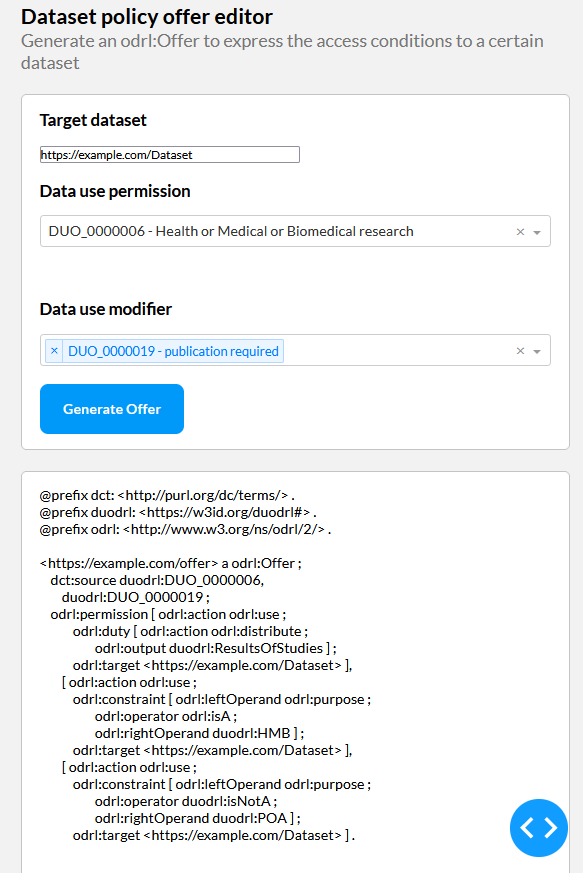
\includegraphics[width=0.4\linewidth]{figures/chapter-6/poc-editor.PNG}}
    \label{fig:editor}
}
\qquad
\subfigure[with OAC and DPV concepts.]{
    \fbox{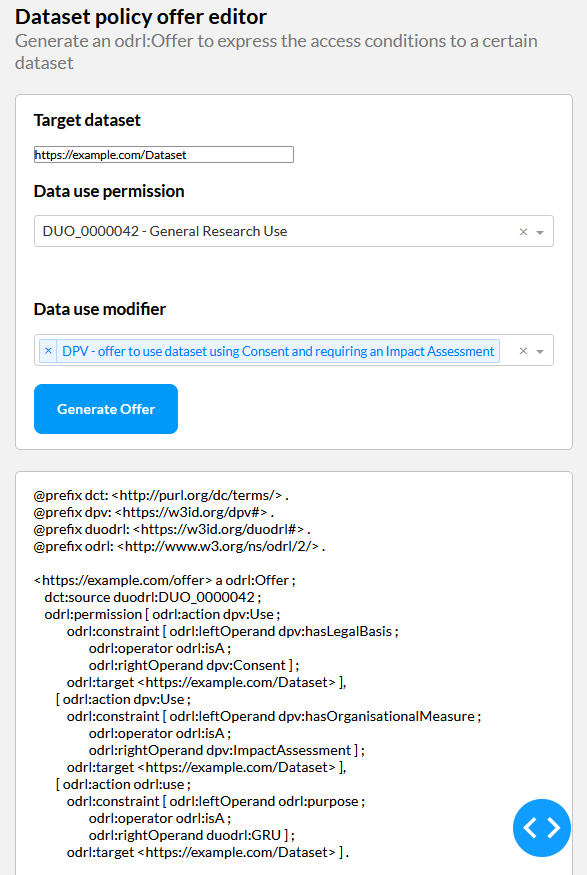
\includegraphics[width=0.4\linewidth]{figures/chapter-6/poc-dpv-editor.PNG}}
    \label{fig:dpv-editor}
}
\end{figure*}

As mentioned in the last Section, the matching algorithm employed in this PoC was adapted from the OAC-based algorithm presented in Section~\ref{sec:algorithm-agreement} to cater to DUO's use case health data-sharing conditions, while ensuring alignment with legal requirements.
During the matching process, the conditions outlined in the request for health data, in the \texttt{odrl:Request} policy, must be compared with those specified in the health datasets' offers, in the \texttt{odrl:Offer} policy.
This entails ensuring that the permissions and prohibitions from the offer instantiation can be met by the request.
Once this compatibility is established, the policies are deemed congruent, a permissive \texttt{odrl:Agreement} is generated, and access can be granted according to the established conditions.
If the policies are not compatible then a prohibitive \texttt{odrl:Agreement} is generated and access to the dataset is denied.
Moreover, for data discovery purposes, the \texttt{odrl:Request} policy needs to be compared against the policies of each available dataset if this PoC is to be implemented within a large-scale system, to ensure that all available datasets and corresponding policies are checked to see if they fit the request.
While pre-computations and optimisations could streamline this process, this is not implemented within this Thesis prototype, as its purpose is solely to serve as a first PoC to test the generation of machine and human-readable data access agreements.

The policy matching algorithm initiates by verifying if a dataset's policy includes a specific rule corresponding to the purpose outlined in the \texttt{odrl:Request}. 
If the dataset's offer has a prohibition for a purpose $P$, access to the dataset may be denied if the request is for $P$; conversely, if a permission is detected, access can be allowed allowed.
Subsequently, as described in the previous Section, similar assessments should be conducted to examine other restrictions beyond purpose, i.e., the ones outlined in Table \ref{tab:DUO_ODRL_overview}, such as constraints on the type of assigner for the agreement, on the location or timing of data use.
In the event of encountering a matching prohibition, access to the dataset must be refused; however, if a permission is present, access may be granted.

If additional obligations are mandated for dataset access and use, such as committing to collaborate with the primary study investigator or providing proof of ethical approval to perform the study, these should included within the \texttt{odrl:Agreement} together with the conditions for access.
In instances where conflicting policies arise from the merge of distinct data use permissions and modifiers, the prohibition supersedes by default, akin to the algorithm's base protocol, established in Section~\ref{sec:algorithm}.
Under such circumstances, access to the dataset is declined.

The outcome of the matching algorithm, an \texttt{odrl:Agreement}, should be generated, incorporating a rule either permitting or prohibiting the solicited \texttt{odrl:Request}, as well as other metadata described in Section~\ref{sec:poc_duodrl}, including linkage with the corresponding \texttt{odrl:Request} and \texttt{odrl:Offer}, and any duties, if specified by the data provider.
In this way, the \texttt{odrl:Agreement} instantiation serves to encapsulate and facilitate the creation of appropriate legal documentation to formalise and communicate the agreement stemming from the submitted request and consequent matching outcome.
The computational overhead associated with generating such an agreement, particularly at a time when the request will be matched against a large number of offer policies, falls outside the scope of analysis of this Thesis.
This is due to the fact that the overhead will vary significantly depending on the use case and on the interpretation of the DUO concepts, which are not explicitly defined and, as such, reflect the specific analysis proposed in this Thesis, aligned with its core foundation on the decentralisation of access to data.
As a result, the focus of this Section is on clearly representing the information through the utilisation of ODRL policies and showcasing the applicability of the proposed OAC-based algorithm for decentralised access to health data on a purpose-based setting, aligned with the legal requirements specified in the GDPR.

%TODO: add figure with screenshot of generated agreement + human readable description

\paragraph{PoC preservation, maintenance, and future improvements}
The PoC implementation is published and archived according to the methodology described in Section~\ref{sec:code_preservation}.
Furthermore, its source code is hosted at \url{https://w3id.org/duodrl/repo}, under the CC-BY-4.0 license.
A live demonstration of the PoC UI features is also available at \url{https://w3id.org/duodrl/app}.
The repository can also be used by DUO/DUODRL users to suggest new features to be added to the PoC, as well as to report bugs through GitHub Issues.
% As future work, SOPE can be extended to include all terms present in the previously mentioned DPV's taxonomies, as well as to cover all constraints defined in the OAC profile, e.g., restrict legal bases or specify the technical and organisational measures used by data controllers to ensure the secure processing of personal data.
% Moreover, with such an extension, SOPE could also be used by data controllers to detail their privacy policies.
% Additionally, user studies should be performed to assess the design choices included in the editor, as well as to understand what type of additional controls people want to have on top of what is legally mandated, e.g., temporal constraints or duties for the data controller to fulfil prior to data access.